\section{The Human Visual System}
\label{sec:background:hvs}
\subsection{The human eye}

\begin{figure}[htpb!]
\centering
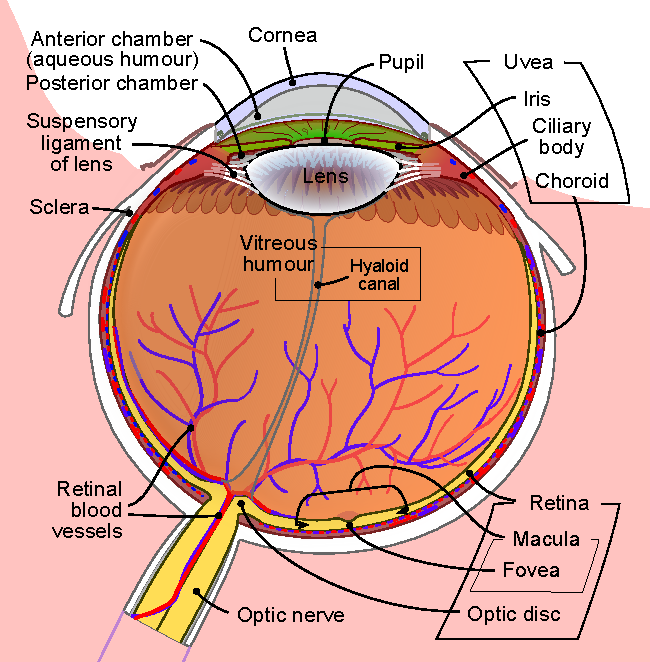
\includegraphics[width=0.59\columnwidth]{images/other/eye_schematic}
\caption[Schematic diagram of the human eye]{Schematic diagram of human eye. Image source: \citet{eyeschematic}}
\label{fig:eye_schematic}
\end{figure}



Fig.~\ref{fig:eye_schematic} shows a schematic diagram of the human eye. 
Light from the external world passes through the pupil and is focused by the lens onto the retina. 
The pupil acts like an aperture stop in cameras. 
The pupil adapts its radius to adjust to the world’s level of brightness, e.g., in a dark room, the pupil’s radius is larger to allow more light into the eye. 
The lens’ shape is deformable by the ciliary muscles. 
The lens’ shape controls the focal length of the eye which in turn determines the distance at which the eye is focussed to.

\begin{figure}[h!]
\centering
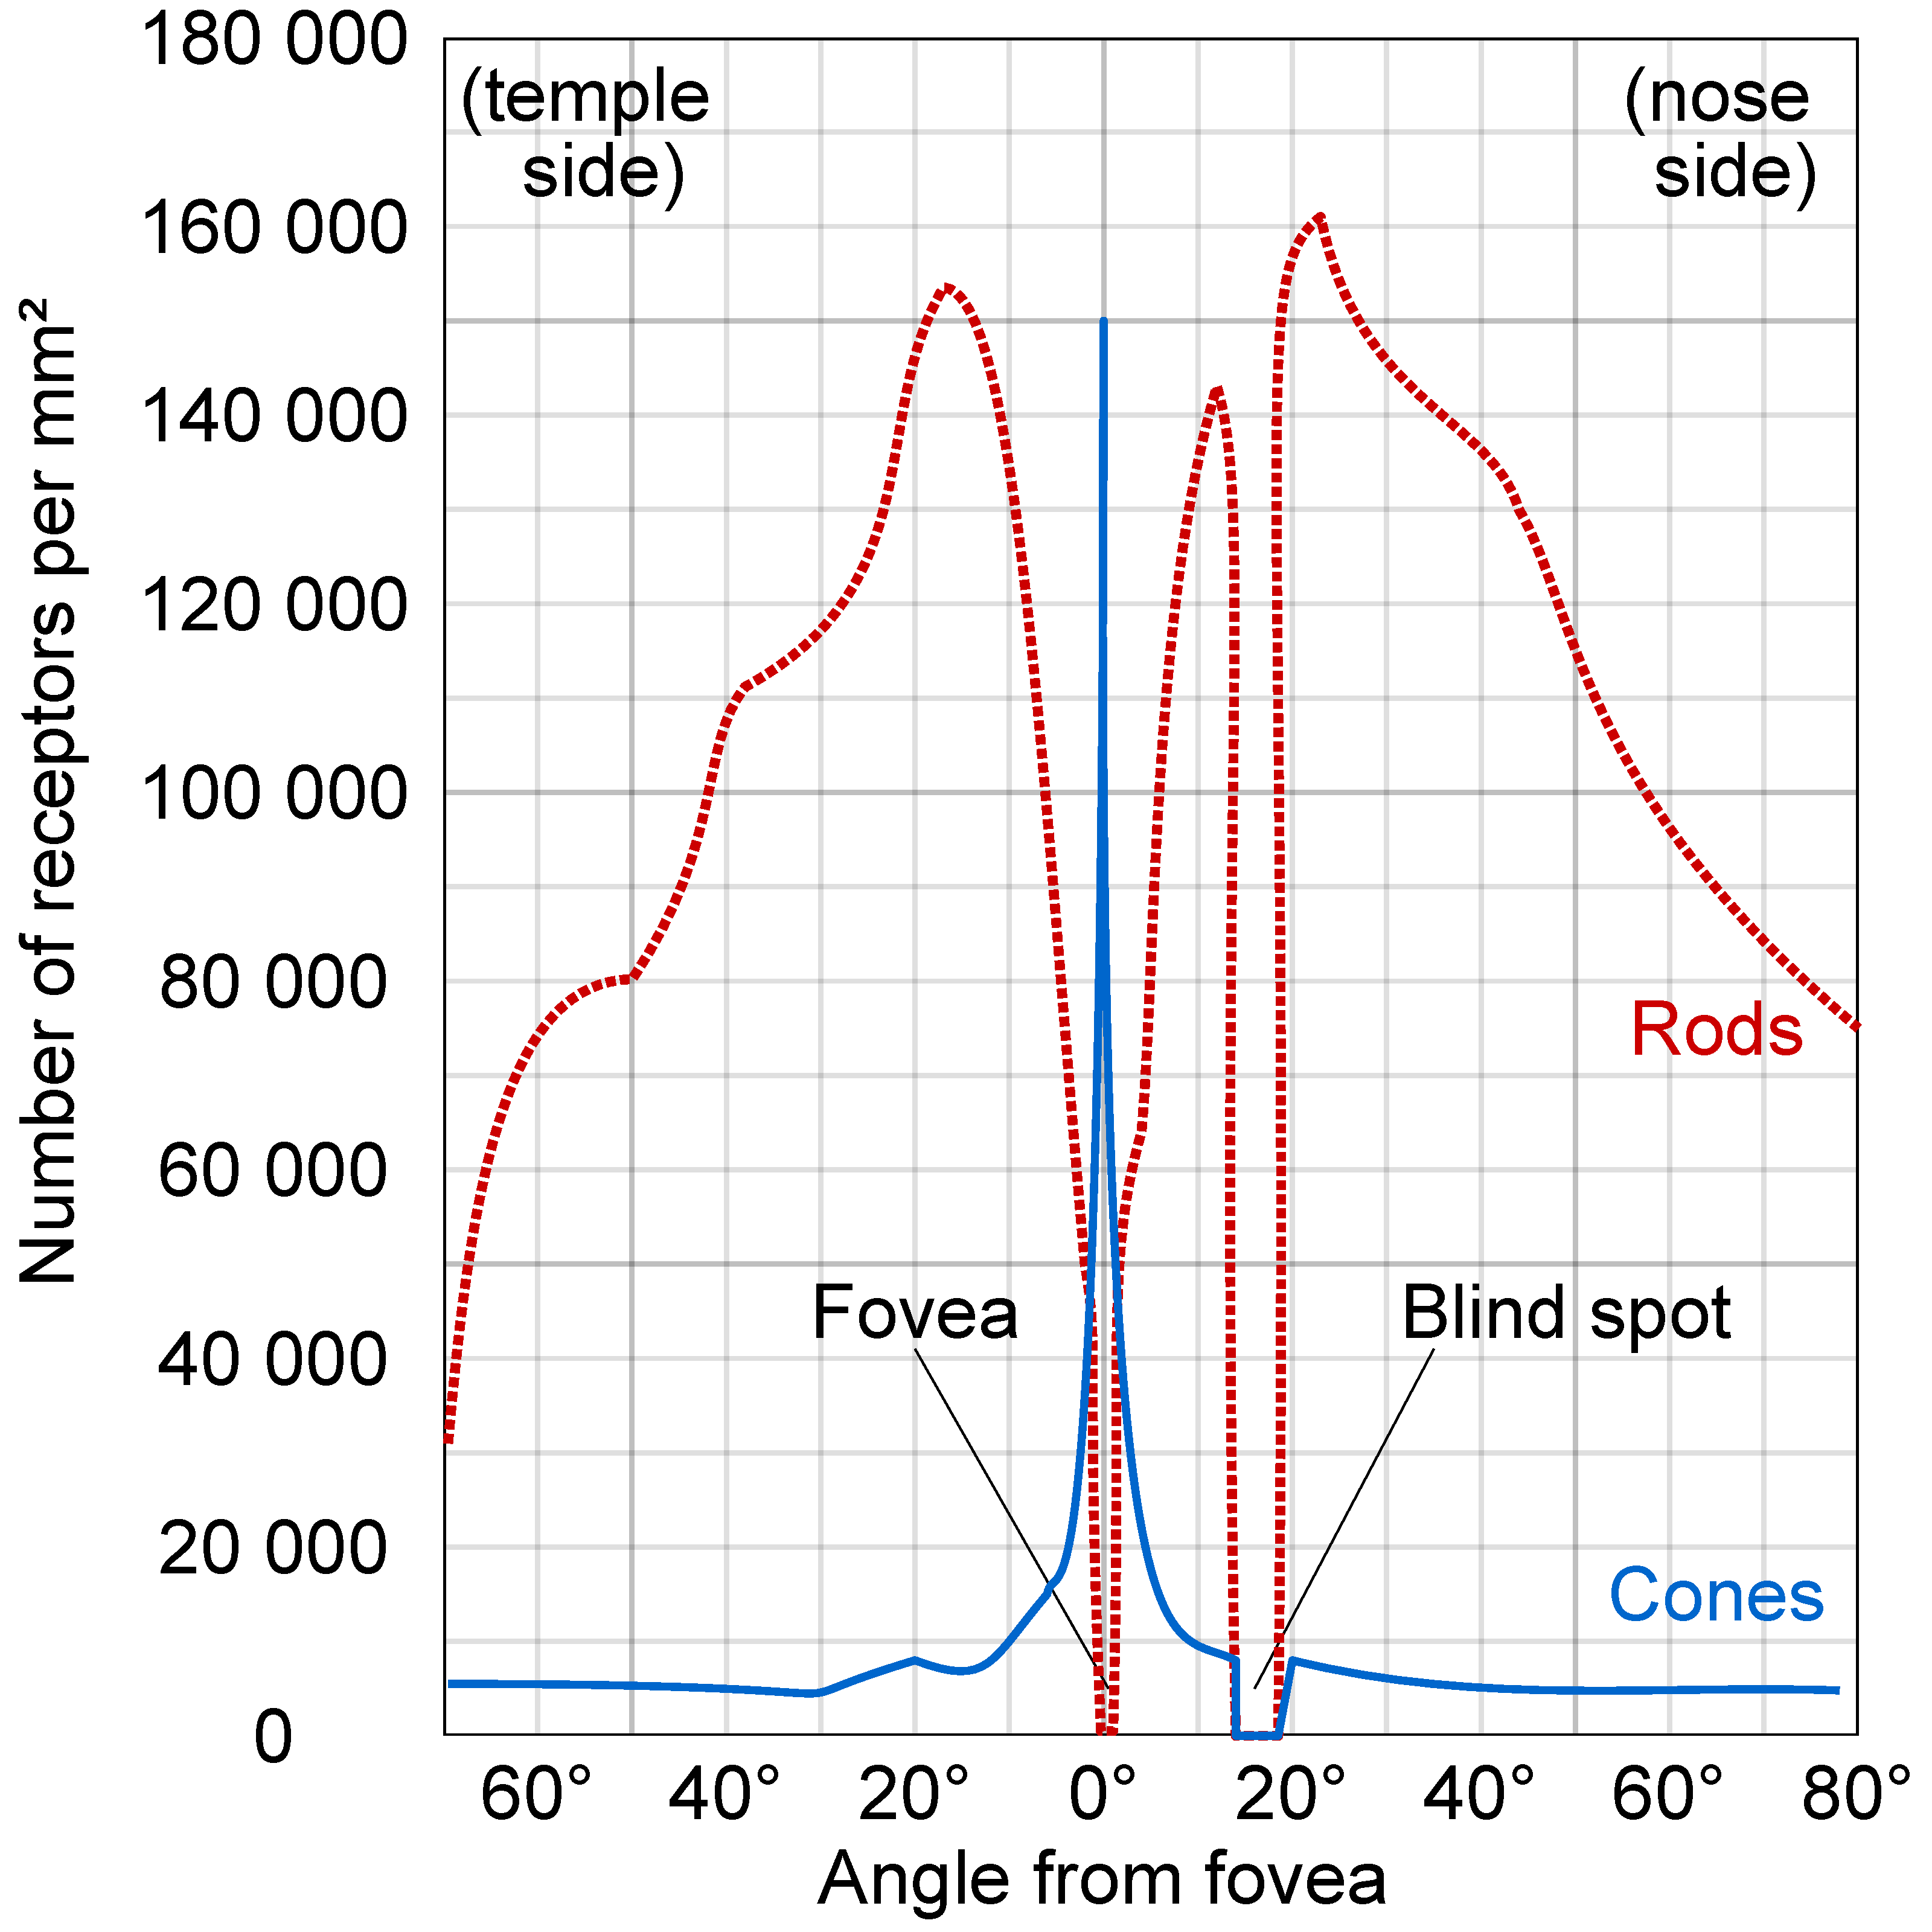
\includegraphics[width=0.59\columnwidth]{images/other/cones_and_rods_distribution}
\caption[Distribtion of rods and cones]{Distribution of rods and cones along a line passing through the fovea and the blind spot of a human eye. Image source:~\cite{conesandrodsdistribution}}
\label{fig:cones_and_rods_distribution}
\end{figure}



Our eye’s retina is composed of two types of sensory cells: cones and rods. 
Cones and rods serve different purposes, e.g., cones are capable of color vision, whereas rods have an achromatic response, but rods are extremely sensitive to light and hence are useful for low-light conditions.
Interestingly, each cone is connected to an optic nerve, but multiple rods share an optic nerve. 
Hence, cones have a higher visual acuity than rods. 
Interestingly, the distribution of cones and rods on our retina is non-uniform. 
Fig.~\ref{fig:cones_and_rods_distribution} shows the distribution of rods and cones. 
Observe how there is a high concentration of cones in a narrow region. This region is called the \emph{fovea}.

\subsection{Depth cues}
\label{sec:background:depth_cues}
\subsubsection{Binocular depth-cues}
Some depth cues that we are aware of depend on information from both eyes. Fig.~\ref{fig:binocular_depth_cues} depicts two binocular depth cues and a brief explanation follows:

\paragraph{Disparity} Since our eyes are at slightly different positions, the image seen by them is also slightly different. 
This slight shift in the content between the images formed in our eyes is called \emph{disparity}. 

\begin{figure}[h!]
\centering
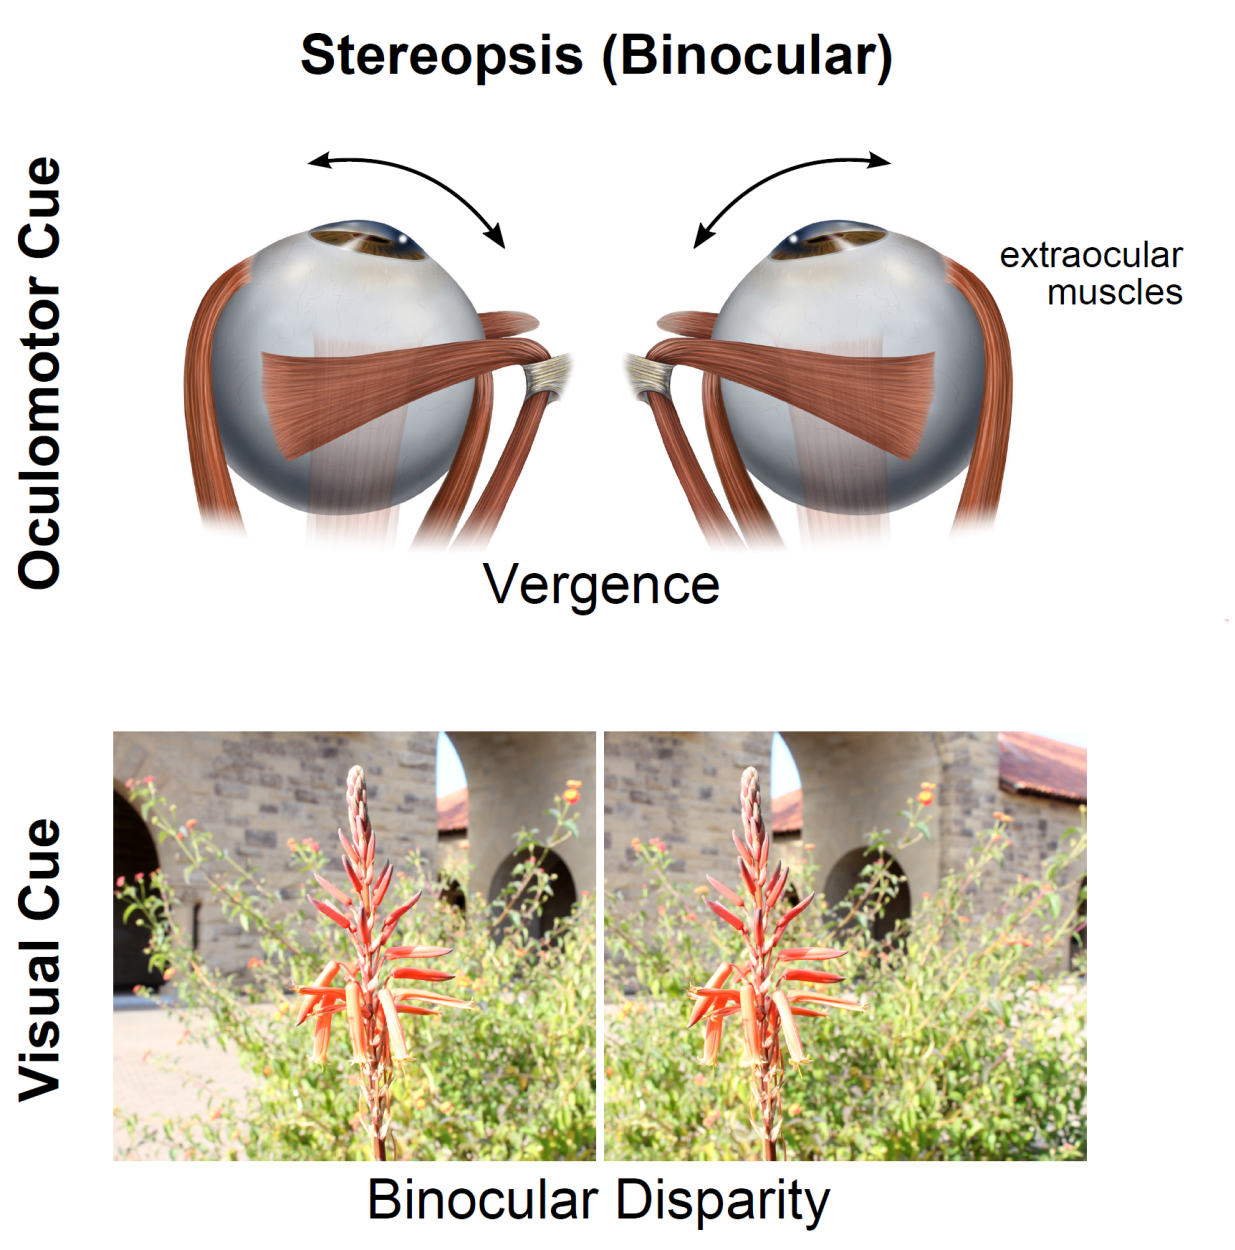
\includegraphics[width=0.59\columnwidth]{images/other/binocular_depth_cues}
\caption[Binocular depth cues]{We perceive depth from these binocular cues (1) \emph{convergence:} our eyes rotate to form the image of the object of attention at our retina, and (2) \emph{disparity:} the images formed in our two eyes are slightly different. Image source: Adapted from \cite{Konrad2017Accommodation}}
\label{fig:binocular_depth_cues}
\end{figure}



The disparity between the images is also dependent upon the depth of the object from the eyes; the closer the object is, the higher the disparity in its image between the two eyes. 

\paragraph{Convergence} When we look at an object, our eyes automatically rotate in such a manner that the image of the object of attention is formed at the fovea. 
The depth of the object determines the angle by which our eyes have to rotate inwards. This depth cue is called \emph{convergence}.

\subsubsection{Monocular depth-cues}
\label{sec:background:monocular}
Depth cues that are available even when the world is viewed with one eye alone are called monocular depth cues. 
There are several monocular depth cues, namely: \emph{occlusion, accommodation, defocus-blur, intrapupillary occlusion, chromablur,} etc. 
We discuss each of these monocular depth-cues below: 

\paragraph{Accommodation} Our eyes have a narrow opening called the pupil to let in light from the world. 
Our eyes have a lens behind the pupil which can be deformed to change the focal distance of the eyes. 
Our eyes automatically try to bring the object of attention into sharp focus on the retina by deforming the lens. 
This ability to change the focus is called accommodation and it provides us with an estimate of the distance. 

\paragraph{Retinal blur} A given lens state fixes the focal distance and brings objects at that focal distance into sharp focus at the retina, but makes objects at other distances blurred. 
This is a property that can be observed in any single-lens imaging system. 
While this retinal blur is a natural phenomenon for real-world scenes, some display technologies that can change the focal distance need to additionally and synthetically blur virtual objects that are away from the focal distance, e.g., varifocal displays. 
\paragraph{Occlusion} Occlusion is a relative depth order cue which arises when the nearer object partially obstructs the view of a farther object. 
Occlusion actually only informs us about the depth ordering and is not useful to estimate the magnitude of depth. 

Such depth cues, which only provide information about the depth order (relative depth) instead of a quantitative estimate of the depth, are called nonmetrical depth cues. 
Other depth cues discussed so far (disparity, convergence, accommodation, retinal defocus) provide a quantitative estimate of the depth and are called metrical depth cues. 

\begin{figure}[h!]
\centering
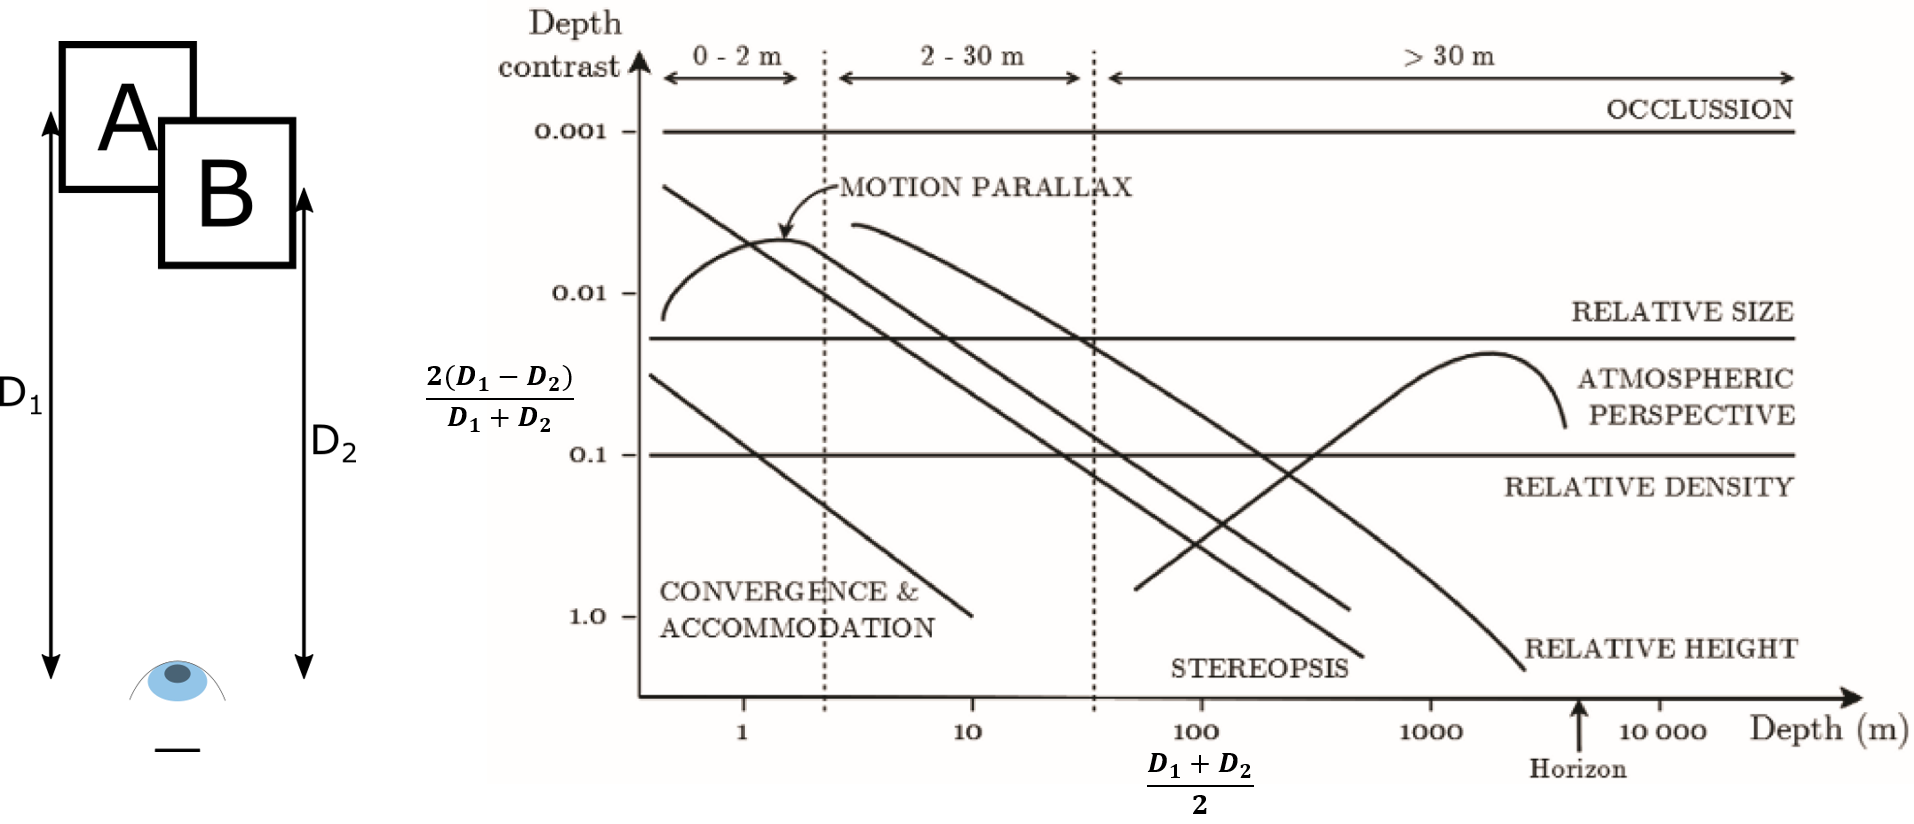
\includegraphics[width=0.99\columnwidth]{images/other/cutting_and_vishton}
\caption[Relative importance of depth cues]{Figure shows the relative importance of different depth cues. Source: Adapted from \citet{cutting1995perceiving}}
\label{fig:cutting_and_vishton}
\end{figure}



Even though occlusion is a nonmetric depth cue, it is nonetheless the most important depth cue. 
In \cite{cutting1995perceiving}, an experiment was done where two objects A and B are shown at different depths, say D1 and D2, and the user is then asked to make a forced-choice as to which object is closer. 
To study the effect of different depth cues, various trials were conducted with only a few depth cues active in insolation. 
And the results of the experiments are summarized by the graph shown in Fig.~\ref{fig:cutting_and_vishton}. 
The horizontal axis of Fig.~\ref{fig:cutting_and_vishton} shows the average distance of the two objects, i.e., $\frac{D_1 + D_2}{2}$ and the vertical axis shows the depth contrast between the two objects, i.e., $\frac{2\left(D_1 + D_2\right)}{D_1 + D_2}$.
And each curve shows minimum depth contrast required for correct ordering at a given depth and given depth cue. 
We can see that for occlusion, the depth contrast can be very low, and we’d still be able to order the objects correctly. 

\paragraph{Other monocular depth cues} There are many more monocular depth cues, e.g., some recently studied ones such as chormablur~\cite{cholewiak2017chromablur}, intra-pupillary occlusions~\cite{zannoli2016blur}, and depth cues that have been known for a long time such as motion parallax, relative size, atmospheric perspective, etc. 
Of the above depth cues, except for chromablur and intra-pupillary occlusions, all depth cues are reproduced accurately by the standard graphics rendering pipeline. 
For chromablur and intra-pupillary occlusions, the displays have to be built either with special optics or non-standard rendering algorithms or both. 
However, chromablur and intra-pupillary occlusions are not as dominant as accommodation, retinal blur, or occlusions.

\section{Beyond 2D Displays}
\label{sec:background:beyond_2d_displays}
In this section, we discuss the approaches to extend the virtual world beyond the traditional 2D displays. 
There are mainly three approaches: (1) 3D displays, (2) shader lamps, (3) Near-Eye Displays. 
Here’s a brief description of each approach:

\subsection{3D Displays}
\label{sec:background:3d_displays}
These displays often resemble the form-factor of traditional computer monitors and present virtual scene with 3D depth cues by presenting each eye with viewpoint-dependent imagery. 
Typically, these displays present only binocular cues. 
These displays sometimes time-multiplex the imagery between the two eyes in synchronization with shutter-glasses. 
Instead of using shutter-glasses, other techniques have been developed that try to re-create the lightfield of the target 3D scene either by using stacks of transparent displays or other novel optical and mechanical configurations. 
With respect to our goal to seamlessly combine the physical and digital worlds, this approach’s main limitation is that the imagery is confined to a local volume or field-of-view.

\subsection{Shader Lamps}
\label{sec:background:shader_lamps}
These systems projectors to display virtual worlds onto physical surfaces such as walls, tables, etc. 
Multiple cameras are used to track the physical surfaces and user interactions. 
Disadvantages with these systems include 
(1) lack of monocular depth cues, 
(2) shadows cast by objects and users pose a difficulty for both projectors and cameras, 
(3) ambient lighting of these specialized rooms needs to be controlled carefully.

\subsection{Head-Mounted Displays}
These are compact and lightweight devices that can be worn on the head and present imagery to each eye. 
These displays are the most promising direction for Augmented Reality because the imagery shown in these displays need not be confined in volume or to any real-world surface. 
However, there are a number of challenges and approaches for Head-Mounted Displays, which are covered in the remainder of this chapter.

\section{Head-Mounted Displays}
NEDs are broadly of two categories, Virtual Reality Displays and Augmented Reality Displays. 
We briefly discuss each category before focussing on just Augmented Reality displays.

\subsection{Virtual Reality Displays}
\label{sec:background:vr_displays}
In Virtual Reality, the user is immersed in a completely synthetic environment and is a useful modality in some scenarios, e.g., immersive movies, immersive training for unusual scenarios, or even computer games. 
While useful in specific scenarios, interaction with the real-world is often unavoidable. 
Hence, it is unlikely that users would be willing to be completely cut-off from the real-world for extended periods of use. 
Therefore, it is difficult to imagine VR as the next productivity tool or computing platform.

\subsection{Augmented Reality Displays}
\label{sec:background:ar_displays}
Augmented Reality NEDs insert virtual objects into the view of the real-world. 
The user maintains the context of the real-world, and the inserted virtual objects are often contextual and spatially registered with the real-world.

\subsubsection{Video see-through AR dislays}
\label{sec:background:vst_displays}
One proposed technology for AR displays is to use a VR display, but relay the real-world’s view using outward-facing camera(s). 
This approach solves the occlusion problem trivially, however, this approach has a major limitation being that the view of the real-world is limited by the display’s and the camera’s resolution (spatial and angular), latency, dynamic range, distortions, field-of-view, and color fidelity. 
In other words, for a video see-through AR display to recreate the same experience of viewing the real-world without the display, camera technologies and display technologies need to advance significantly.

\subsubsection{Optical see-through AR displays}
\label{sec:background:ost_displays}
Optical see-through AR displays optically insert virtual imagery into the user’s view of the realworld. 
Of all the display technologies that seek to integrate the real-world and the virtual world, only optical see-through AR displays propose to do in a portable manner and with minimum encumbrance to the real-world view.

\subsection{Similarities and Differences between Virtual Reality and Augmented Reality}
\label{sec:background:ar_vs_vr_displays}

Augmented Reality and Virtual Reality are similar technologies in these respects: the need for presenting imagery with optics placed close to the eye, the need for head and eye tracking, and a similar rendering and display graphics pipeline, etc. 
However, there are also differences in the enabling technologies:

\begin{enumerate}
    \item The additional need for an occlusion mask for AR displays to depict opaque virtual objects
    \item Since a VR display completely blocks out the real world, the user’s own body can not be seen naturally. It would be necessary to 3D reconstruct the user’s body and display it within the virtual scene in real-time.
    \item For spatially registering virtual objects to the real world, it is often necessary to 3D reconstruct the real-world in real-time.
    \item More stringent design requirements for AR displays, e.g., AR displays should not encumber the view of the real-world (can not have on-axis components that distort or block the real-world), need lower display latency for virtual objects to appear registered to the real-world, display needs to support a wider range of brightness levels, etc. 
\end{enumerate}

\section{Requirements for Augmented Reality Displays}
\label{sec:background:requirements_ar_displays}
The below requirements are arranged approximately in the descending order of subjective importance of the author.

\begin{enumerate}
    \item \textbf{Compact form-factor:} Future AR headsets may consist of the display unit, multiple sensors (head and eye tracking, cameras for 3D reconstructing the environment, inertial measurement units (IMU)), computing units (CPU and GPU), communication units, and a battery. Despite integrating all these components, it is important that these devices are lightweight so that the users can wear these devices for long hours. \cite{yan2018effects} recommend that VR headsets should be designed with uniform weight distribution and aim to keep the weight within 300 g.
    \item \textbf{Wide Eyebox:} Eyebox refers to the range of pupil positions from where the virtual image presented by the AR display can be seen. The eyebox is the same as the exit-pupil of the display. Many display technologies and prototypes have been demonstrated which have beautiful imagery but with narrow eyeboxes~\cite{Maimone2017Holographic,westheimer1966maxwellian}. For such displays, eyebox replication techniques are quite useful~\cite{Jang2017Retinal}. 
    \item \textbf{Wide Field of view:} The human visual system has a monocular field-of-view of about 120 degrees and a binocular field of view of about 210 degrees. To effectively integrate the real and digital worlds, AR displays should aim to present wide field-of-view imagery.
    \item \textbf{High Resolution:} The human visual system is capable of viewing resolution as high as 60 cycles-per-degree. However, the human visual system has such a high resolution only for a narrow region on the retina called the fovea. Beyond this region, the resolution drops drastically and is very low in the peripheral field-of-view. This non-uniform resolution across the field-of-view provides an opportunity to provide high-resolution imagery without having to build very high-resolution display panels but poses a challenge to dynamically change the display as the eye looks in different directions.
    \item \textbf{Depth cues:} AR displays should provide depth cues similar to that available in the real world. The various depth cues that the human visual system uses are discussed in Sec.~\ref{sec:background:depth_cues}. 
    \item \textbf{Low Latency:} AR displays need to respond fast to the user’s head and eye movements by updating the imagery being displayed. It is estimated that even 10 milliseconds delay between head motion and display update can result in 5 centimeters of error for a virtual object situated at 2 meters away. See Appendix~\ref{sec:appendix:registration_errors_latency} for the calculation behind these numbers.
\end{enumerate}
A more detailed description of Augmented Reality and its requirements are covered by these review papers: \cite{azuma2001recent,carmigniani2011augmented}. 

\section{Overview of previous work for depth cues in AR displays}
\label{sec:background:previous_work_ar}
Current commercially-available AR displays offer impressive capabilities, but they typically do not support important monocular depth cues such as accommodation or occlusion, resulting in a transparent image overlaid onto the real-world at a fixed depth. 
To realize the vision of Augmented Reality, providing a seamless and perceptually realistic experience requires displays capable of presenting photorealistic imagery, and especially, perceptually realistic depth cues, resulting in virtual imagery being presented at any depth and of any opacity. 
Previous research prototypes fall short by presenting occlusion only for a fixed depth, and by presenting accommodation and defocus-blur only for a narrow depth-range, or with poor depth or spatial resolution. 
We briefly discuss major themes in previous work for addressing the lack of accommodation and depth-dependent occlusion. 
Later, in each technical chapter (Chapter \ref{chapter:volumetric_ned} and \ref{chapter:varifocal_occlusion_ned}), a detailed review of previous work is presented in context for the technology presented in that chapter.

\subsection{Accommodation}

Previous AR displays that propose technologies to provide accommodation are broadly classified, and their limitations are mentioned:

\begin{enumerate}
    \item \emph{Varifocal Displays:} \cite{Dunn2017Wide,Aksit2017Near} Provides synthetic focus cues, requires to track accommodation-state of the eye, and has latency in moving the in-focus plane.
    \item \emph{Multifocal Displays:} \cite{Akeley2004,Narain2015optimal} Few focal planes which leads to partly synthetic focal cues and reduced spatial resolution for content in-between the few focal planes.
    \item \emph{Light-field Displays:} \cite{Maimone2014Pinlight} Poor spatial resolution, frame-rates, and narrow depth-range. 
    \item \emph{Holographic Displays:} \cite{Maimone2017Holographic} Very small eyebox, narrow depth-range.
\end{enumerate}

\subsection{Occlusion}

\emph{Fixed-focus occlusion displays} \cite{Kiyokawa2000,Kiyokawa2001,Kiyokawa2003} can preserve a high-quality of the see-through view, but present the occlusion mask at a fixed distance. 

\emph{Light-field occlusion displays} \cite{maimone2013general} attempts to provide depth-dependent occlusion by presenting a 4D light field occlusion mask using stacked LCD layers placed out of focus in front of the eye, where the occluding patterns are calculated by light field factorization algorithms \cite{Lanman2010,Wetzstein2012}. 
While theoretically capable of presenting depth-dependent occlusion cues, this approach’s use of LCD panels causes severe diffraction and deterioration of the real-world’s view. 

